\chapter{Computational Methodology}

\label{ch:compmethodology}

\section{Density functional theory}

Quantum mechanics is the most complete modern theory which describes the behaviour of matter at the energy scale of atoms. It can be used to predict things such as the energy levels of atoms, the interactions of light with matter accurately, and the thermodynamic stability of systems of atoms. Ideally, the mathematical formalisms of quantum mechanics would be used to predict the properties and behaviour of all possible types of molecules and materials. In reality, this is very difficult to achieve, requiring several approximations and abstractions in order to produce a method which, in the end, sacrifices physical accuracy in order to be computationally tractable. The most successful field of study in this domain for most solids is that of density functional theory.
% The mathematical formalisms of quantum mechanics must themselves be discretised to be used in computational simulation methods.

\subsection{The Schr\"{o}dinger equation}



\begin{equation}
E\Psi(\textbf{r}) = \hat{H}\Psi(\textbf{r})
\label{equation:schrodinger}
\end{equation}

Where $E$ is the total energy of the system, $\Psi$ is the wave function, and $\hat{H}$ is the energy Hamiltonian operator which includes the kinetic energy contributions ($\hat{T}$) and potential energy contributions ($\hat{V}$), shown in atomic units in equations \ref{equation:kineticcontribution} and \ref{equation:potentialcontribution} respectively:

\begin{gather}
\hat{H} = \hat{T} + \hat{V} \label{equation:hamiltonian}\\
\hat{T} = -\sum_i{\frac{1}{2}}\nabla^2_{r_i} - \sum_i{\frac{1}{2M_i}}\nabla^2_{R_i} \label{equation:kineticcontribution} \\
\hat{V} = \sum_{i,j=i+1}{\frac{1}{2|r_i - r_j|}} + \sum_{i,j=i+1}{\frac{Z_i Z_j}{2|R_i - R_j|}} - \sum_{i,j}{\frac{Z_i}{2|R_i - r_j|}} \label{equation:potentialcontribution}
\end{gather}

where $r_{i}$ is the position of electron $i$, $R_{i}$ is the position of nucleus $i$ and $M_{i}$ is the mass of nucleus $i$. Thus, the second term on the right of equation \ref{equation:kineticcontribution} relates to the kinetic energy of any associated nuclei, and the first term to electrons.

\subsection{Kohn-Sham Method}

Density Functional Theory (DFT) was developed by Kohn and Sham in 1964 \cite{Kohn1965} as an ab initio method for solving the wave equation. The Kohn-Sham Hamiltonian (Equation \ref{equation:kohnsham}) is used in the Schr\"odinger equation.

\begin{equation}
\hat{H}(\rho(\textbf{r})) = E_{KE}(\rho(\textbf{r})) + E_{P}(\rho(\textbf{r})) + E_{XC}(\rho(\textbf{r}))
\label{equation:kohnsham}
\end{equation}

Where $E_{KE}$ and $E_{P}$ are the kinetic and potential energy functionals (functions of functions), $\rho$ is the electron density, $E_{XC}$ is the exchange correlation functional, and \textbf{r} is the position vector. The main approximation is to consider that the electrons only interact with nuclei and the average field generated by all other electrons, and not other electrons explicitly, thus allowing all the terms to be evaluated using the electron density rather than position. An exchange correlation term is then used to include the non-classical electron-electron interactions, namely electron exchange and correlation. Additionally, the exchange correlation term also includes the difference in kinetic energy found due to the use of non-interacting electrons. While Kohn and Sham did provide a proof for the existence of an exchange correlation function, a general form of the functional has not yet been found, although several forms have been considered, each with their own strengths and weaknesses when applied to different systems. One basic form of the functional which is frequently used is the local density approximation (LDA) CITATION XXX:

\begin{equation}
E_{LDA}(\rho(r)) = [integral]\rho(r)E_{uniform}(\rho(r))dr
\label{equation:LDA}
\end{equation}

where $\rho(r)$ is the electron density at location $r$, and $E_{uniform}$ is the exchange-correlation energy of a uniform electron gas (an idealised system). This exchange-correlation functional generates accurate results in materials such as metals where the electron density is relatively uniform, while systems with more variable electron densities (e.g. highly ionic materials) require more complex functionals. A natural extension of the LDA is to also take into account the gradient of the electron density, thus allowing a smoother functional fit when electron density is highly variable with position. Such functionals are collectively referred to as generalised gradient approximations (GGAs). One GGA which has enjoyed widespread use for many different types of systems is the Perdew-Burke-Ernzerhof (PBE) GGA. The accuracy of this functional when modelling solid phase systems is well-established, and its frequent use in DFT studies provides ample reference material for comparing results. After conducting several convergence tests (see \ref{section:convergence}), the PBE GGA was chosen as the exchange-correlation functional to be used for all calculations in this work.

\subsubsection{Born-Oppenheimer approximation}

The Born-Oppenheimer approximation is a two-step process for evaluating atomic forces, which greatly reduces the computational costs of any atomistic simulation. It exploits the large difference in mass between nuclei and electrons in order to separate their interactions. This allows us to decompose the total wave function into a product of an electronic wave function and a nuclear wave function via a separation of variables approach. The first step involves ignoring the kinetic energy contribution of nuclei by assuming they are stationary, thus we can remove the nuclear kinetic energy term in Equation \ref{equation:kineticcontribution}. The stationary nuclei assumption also simplifies the nuclear-nuclear Coulombic repulsion term in Equation \ref{equation:potentialcontribution} because $|R_i - R_j|$ becomes a constant throughout the calculation. An electronic Schr\"{o}dinger equation is then solved where electronic positions are variables and nuclear positions are fixed parameters. This solution contains information of the shape of the electronic orbitals. The next step is to take the electronic distribution and calculate the resultant forces on the nuclei. The nuclear positions are then modified to try to minimise these forces, followed by feeding these nuclear positions back into the electronic Schr\"{o}dinger equation to obtain the new electronic distribution. This process is repeated until the required convergence criterion (energy change per iteration, forces on nuclei) are satisfied.

\subsection{Pseudopotentials}

The electron-electron interaction component of the potential energy presents a problem when it comes to scaling experimental models. The number of terms in this interaction grows quadratically with the number of electrons in the system, and quickly becomes computationally intractable for even small systems. However, we know that in chemical reactions, the majority of chemical behaviour is determined by relatively few valence electrons, while the more numerous core electrons have a far smaller effect. Consider the zirconium atom with 40 electrons, of which 4 (4$d^2$5$s^2$) are typically involved in bonding and chemical reactions. By only considering only these valence electrons for Coulombic-term calculations, we reduce the system size by 90\% which provides much more than a tenfold reduction in computational requirements. Although the core electrons do not participate in chemical reactions, they still influence the properties of the atom, such as the atomic radius. Instead of modelling the core electrons explicitly, we can approximate their aggregate effect with a potential energy function. This is what we aim to achieve by using the pseudopotential method. An example pseudopotential is shown in figure \ref{figure:pseudopotential}.

\begin{figure} % Pseudopotential Image
\label{figure:pseudopotential}
\begin{center}
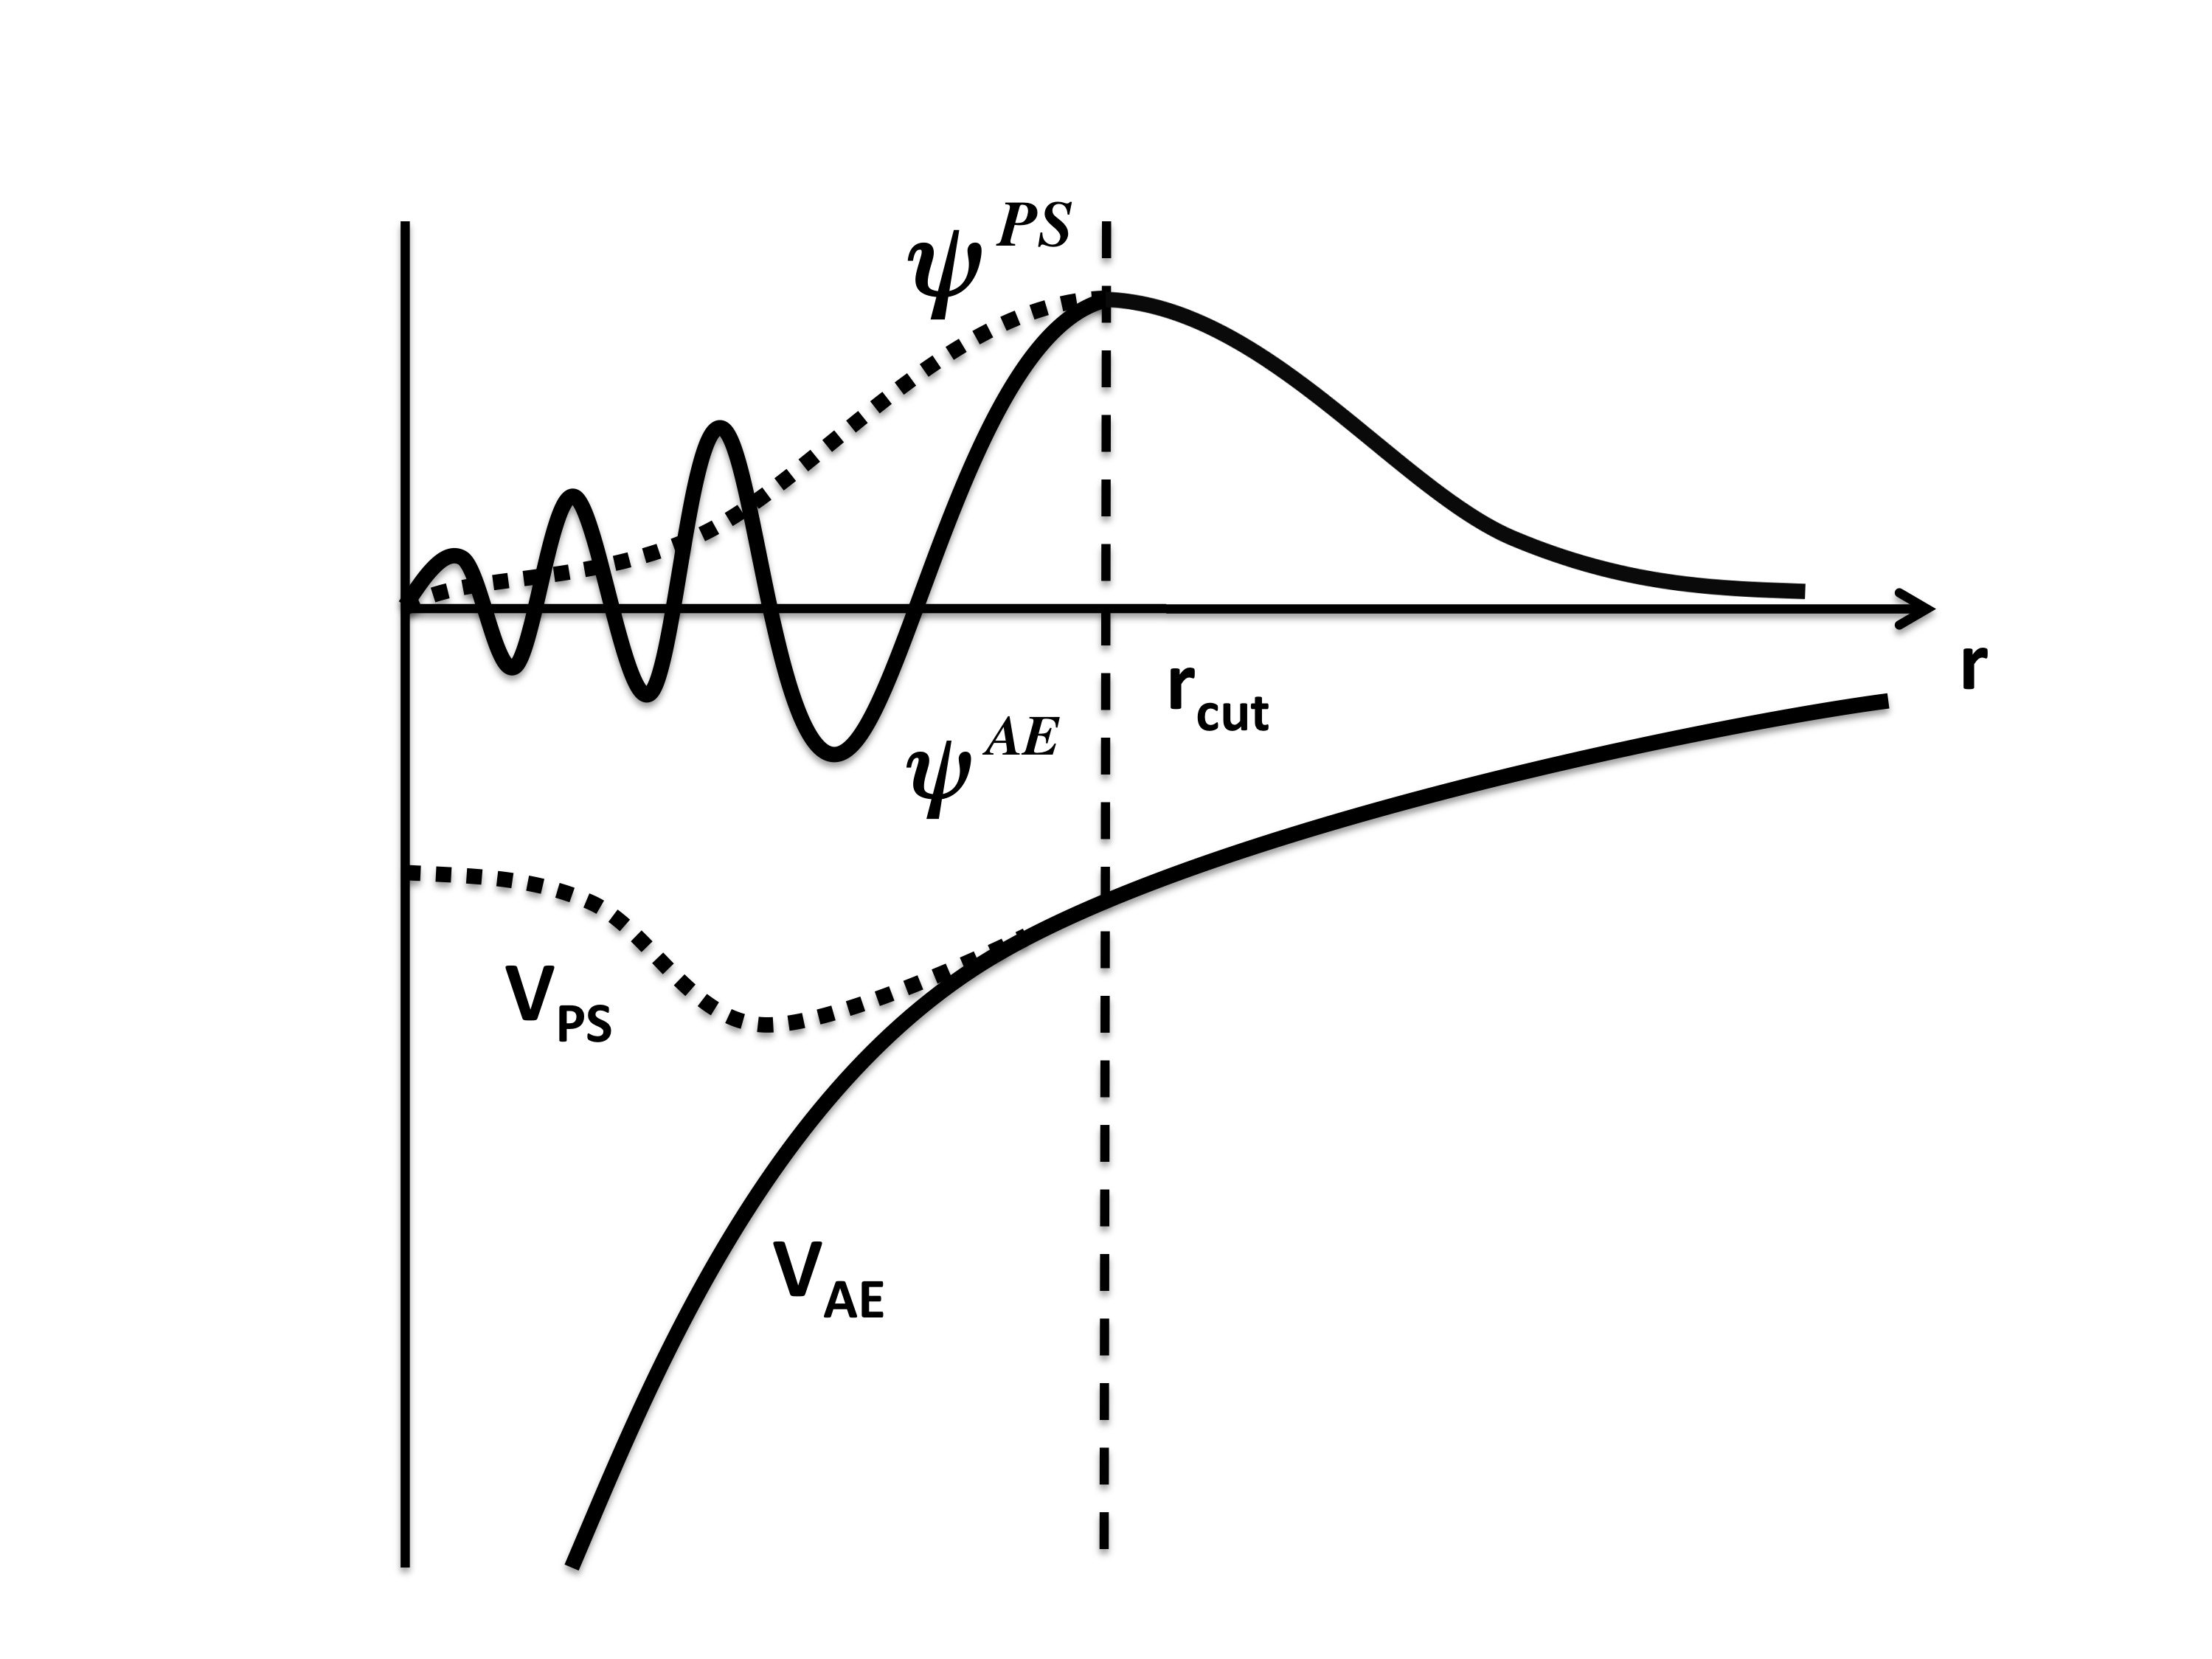
\includegraphics[height=10cm]{images/pseudopotential.png}
\end{center}
\caption{Illustration of an all-electron potential V$_{AE}$ and a pseudopotential V$_{PS}$ with their corresponding wave functions. r$_{cut}$ indicates the radius beyond which both the potentials and their wave functions are the same. Taken from \cite{Payne1992}.  }
\end{figure}


Figures \ref{figure:oxygen_pseudopotential} and \ref{figure:zirconium_pseudopotential} show the actual pseudopotentials used throughout this work for oxygen and zirconium respectively. The potentials are shown broken down by the electronic sub-shells occupied by the valence electrons.

\begin{figure} % Oxygen pseudopotential
\label{figure:oxygen_pseudopotential}
\begin{center}
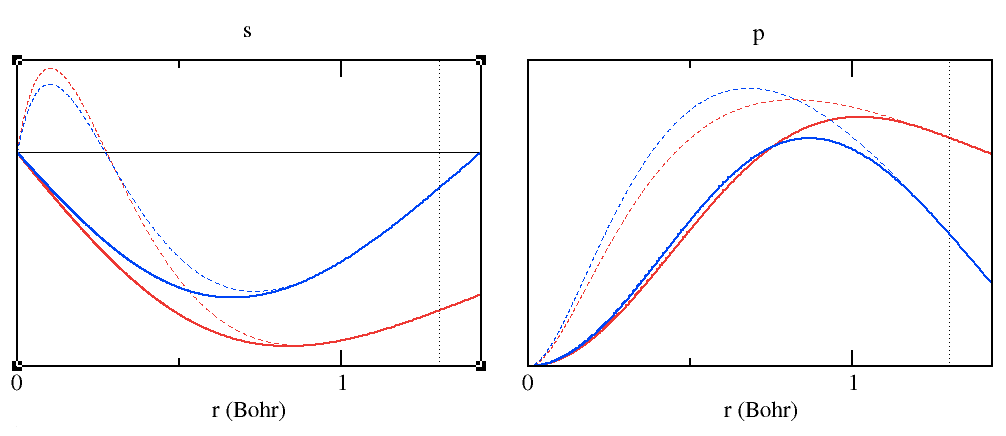
\includegraphics[height=7.3cm]{images/oxygen_otf_pp.png}
\end{center}
\caption{Plots of the valence $s$ and $p$ orbital potentials for oxygen. Dashed lines indicate the all-electron potentials while solid lines indicate the corresponding pseudopotential. Dotted vertical line marks the radius beyond which the potentials match.}
\end{figure}


\begin{figure} % Zirconium pseudopotential
\label{figure:zirconium_pseudopotential}
\begin{center}
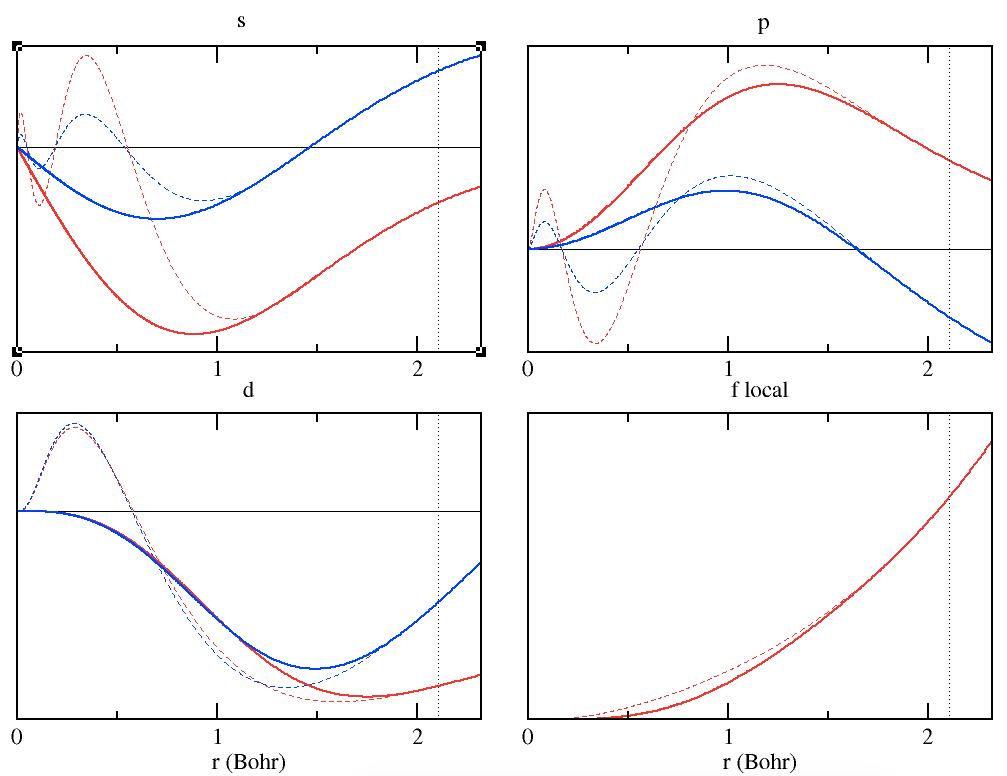
\includegraphics[height=12cm]{images/zirconium_otf_pp.png}
\end{center}
\caption{Plots of the valence $s$, $p$ and $d$ orbital potentials for zirconium. Dashed lines show the all-electron potentials while solid lines indicate the corresponding pseudopotential. Dotted vertical line marks the radius beyond which the potentials match.}
\end{figure}


\section{Periodic boundaries}

\subsection{Bloch's theorem}

The repeating nature of a crystal structure, defined by the lattice vectors plus a basis set of atoms that are repeated, is well-suited for computer models. It allows us to define periodicity in three dimensions for a given unit cell. An example of this periodicity is illustrated in Figure \ref{figure:periodicboundary} in two dimensions. Utilising this periodicity is theoretically justified as follows:

\begin{itemize}

\item Nuclei are arranged in a periodically repeating pattern, thus their potentials acting on electrons are also periodic.

\item If the potential is periodic, it follows that the electron density is also periodic.

\item The electron density is equivalent to the square of the wave function magnitude, thus the magnitude of the wave function is also periodic.

\end{itemize}

Knowing that the magnitude of the wave function is periodic greatly simplifies the calculation process; only one `period' of the function needs to be evaluated. However, the phase of the wave function can take any of an infinite number of values and still satisfy the periodicity condition. At this point, we consider Bloch's theorem which states that the possible wave functions are all quasi-periodic, and thus the wave function can be expressed as in Equation \ref{equation:bloch}:  % Patrick's Fig 2.3 is really useful for describing this

\begin{equation}
\label{equation:bloch}
\psi_k(\textbf{r}) = e^{i\textbf{k}.\textbf{r}}u_k(\textbf{r})
\end{equation}

Where $\psi_k(\textbf{r})$ is the wave function evaluated at position \textbf{r}, $e^{i\textbf{k}.\textbf{r}}$ is an arbitrary phase factor, and $u_k(\textbf{r})$ is a periodic function with the same periodicity as the wave function. Solutions to this equation exist for any value of \textbf{k} and so the general solution can be expressed as an integral over the first Brillouin zone, the primitive lattice cell in reciprocal space. Instead of evaluating the integral over the range of \textbf{k} (a computationally costly task as it is done for many wave functions), a sum of values at discrete points, known as k-points, is used. This approximation is valid because the wave function varies slowly over \textbf{k}, thus allowing the integral to be approximated with several appropriately space k-points. In general, a finer k-point grid results in increased accuracy, but at an increased computational cost \cite{Hasnip2010}.

\subsection{Plane-waves}

Describing the electron density of a system is done in the context of a basis set. A basis set is simply a collection of functions (known as basis functions) which can be combined to produce some relevant output, typically the mathematical description for the shape of an electron orbital. For example, any sound wave can be generated from a combination of sine functions (basis functions). The purpose of a basis set is to describe the varying amplitude of the electron density in space. Any complete basis set (plane-wave, correlation-consistent, split-valence) may be used to represent the behaviour of electron orbitals, but a plane-wave method was chosen due to their greater suitability for periodic systems (plane-waves are intrinsically periodic). 

Figure \ref{Figure:cutoffconvergence} shows the first convergence study where the total energy of simulations with various values of $E_{cutoff}$ were compared to a highly converged value, and then plotted on a log scale to see how precision is improved at larger values.

\begin{figure} % Periodic boundary image
\label{figure:periodicboundary}
\begin{center}
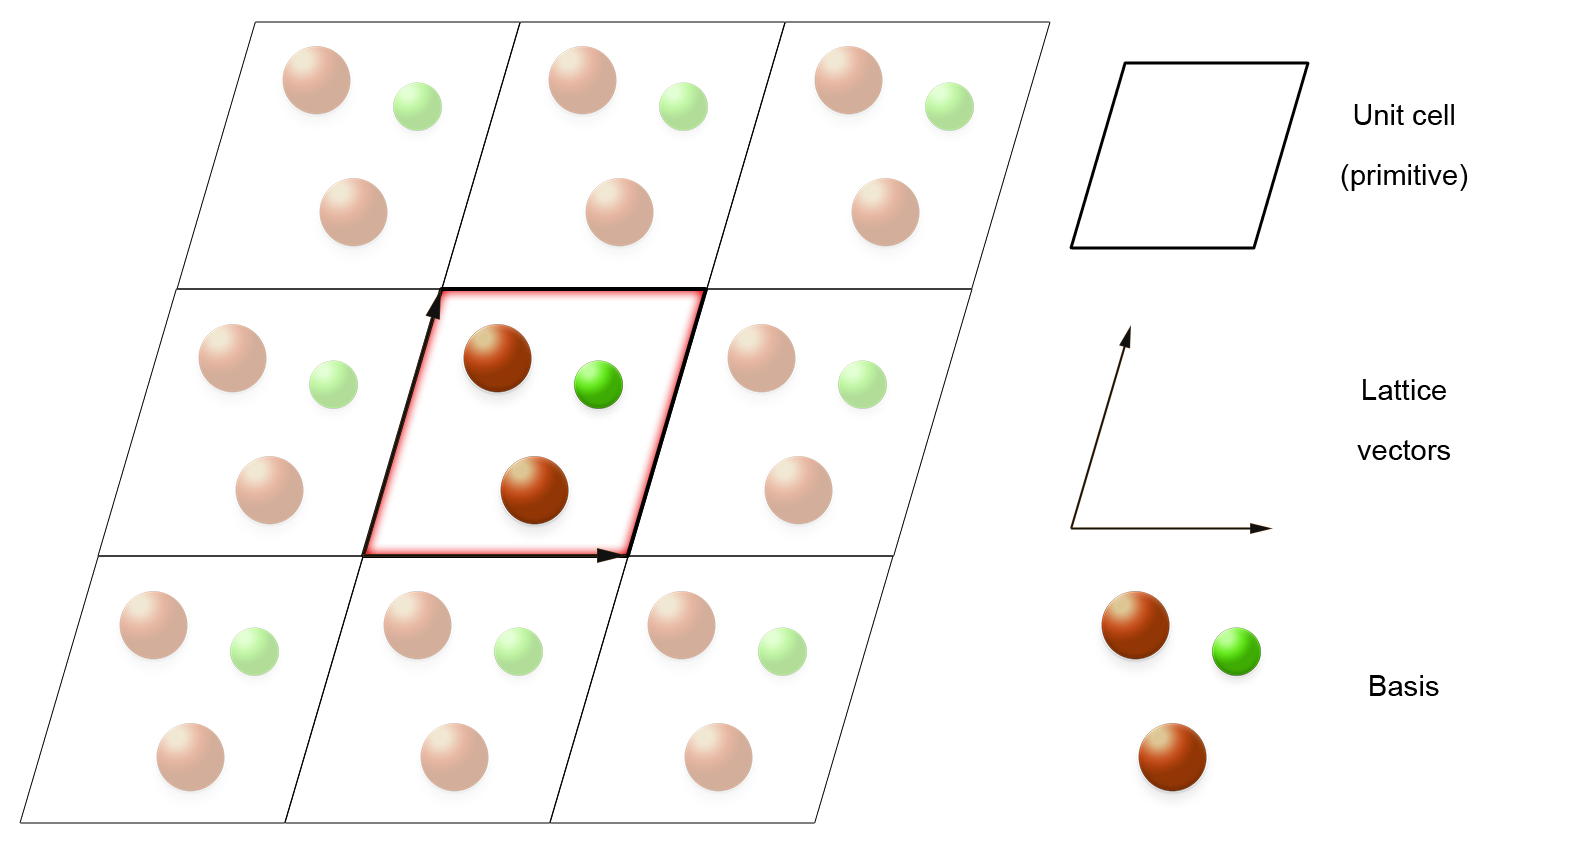
\includegraphics[width=\linewidth]{images/PeriodicBoundaryThesis.png}
\end{center}
\caption{Two dimensional illustration of periodic boundary around a primitive cell.}
\end{figure}


\section{Computational details}
\subsection{Cell dimensions and initialisation}

A supercell method is used for the study of various defects. The first step is to create a unit cell of \zirconia\ in each of the three crystal structures. Each unit cell is then fully relaxed through a geometry optimisation process (see \ref{geometry_optimisation_method}). The resulting cell is then used to construct supercells through tessellation in three dimensions, before being fully relaxed again. This way, we generate systems with up to ten times as many atoms as the unit cell (supercell details can be found in Table \ref{table:supercells}). This is necessary because introducing defects into a small unit cell will result in the defect interacting with itself across the periodic boundary. A supercell increases the distance between the defect and its periodic image, using the bulk material as an interaction buffer. When constructing a supercell, it is important to consider making the supercell equally large in all directions, such that any directional bias in defect-defect interaction is minimised. Larger supercells carry an increased computational cost when running calculations, limiting the sizes we can achieve. For example, a constant-volume defect calculation with 300 atom supercells will take upwards of 500 hours to complete, whereas the equivalent 100 atom supercell will take just 72 hours (fully relaxed calculations are even more computationally expensive).


\begin{table}[ht] % Supercell details
\doublespacing
\centering
\caption{Composition of the supercells in terms of the number of individual unit cells stacked in each direction.} % Unit cells were stacked in such a way as to produce the most cubic supercell in order to minimise directional defect-defect interactions.}
\label{table:supercells}
\begin{tabular}{cccccccc}
\hline
\multirow{2}{*}{{\bf \begin{tabular}[c]{@{}c@{}}Crystal \\ Structure\end{tabular}}} & \multicolumn{3}{c}{{\bf No. unit cells}} & \multicolumn{3}{c}{{\bf Supercell size (\AA)}} & \multirow{2}{*}{{\bf \begin{tabular}[c]{@{}c@{}}No.\\ atoms\end{tabular}}} \\ \cline{2-7}
 & \hspace{0.25 cm} a \hspace{0.2 cm} & b & c & a \hspace{0.0 cm} & b & c \hspace{0.35 cm} &  \\ \hline
\begin{tabular}[c]{@{}c@{}}Monoclinic\\ ($P2_1/c$)\end{tabular} & 2 & 2 & 2 & 10.37 & 10.47 & 10.75 & 96 \\ \hline
\begin{tabular}[c]{@{}c@{}}Tetragonal\\ ($P4_2/nmc$)\end{tabular} & 3 & 3 & 2 & 10.85 & 10.85 & 10.56 & 108 \\ \hline
\begin{tabular}[c]{@{}c@{}}Cubic\\ ($Fm\overline{3}m$)\end{tabular} & 2 & 2 & 2 & 10.22 & 10.22 & 10.22 & 96 \\ \hline
\end{tabular}
\end{table}

\subsection{Geometry optimisation} \label{geometry_optimisation_method}

The geometry optimisation task in CASTEP follows a simple steepest-descent algorithm which attempts to satisfy certain convergence criteria, depending on the constraints applied to the system. This is an iterative process which takes an initial system state, modifies ion positions slightly and then calculates the difference in properties between the states to check for convergence. The variational principle in quantum mechanics tells us that the lowest system energy calculated is always an upper bound for the ground state energy, thus providing a quick and easy way to check if modifications to the system are actually optimising the geometry. The exception is when the system converges upon a local minima which may or may not be an experimentally observed state. This can be avoided to some extent by having good initial ion placement to optimise from.


\subsection{Convergence criteria for geometry optimisation}

Four convergence criteria are used for the geometry optimisation tasks throughout this work, one of which is only used when performing constant-pressure calculations, such as when a supercell is being fully relaxed. These criteria are evaluated with respect to the previous iteration during the geometry optimisation task:

\begin{itemize}
\item \emph{Change in energy per ion} : The largest change in the energy per ion between iterations must be below $10^{-5}$ eV. Below this value, the total energy improvement towards the ground state for a 100 atom supercell is less than 0.001 eV, and is therefore considered converged.
\item \emph{Maximum force on an ion} : The maximum force requirement on any single ion in an iteration must be below $10^{-2}$ eV/\r{A}. This is required to make sure that the ion position will not change significantly in the following iteration, possibly bringing another convergence criterion above its threshold.
\item \emph{Maximum change in ion position} : This must be below $5 \times 10^{-4}$ \r{A} between iterations to be considered converged. This criterion specifies the maximum `rattle' of the ion that is tolerated once the minimum energy is reached (i.e. displacements above this value may still be important for achieving a correct atomic configuration). 
\item \emph{Maximum stress (constant-pressure only)} : During unconstrained relaxation, the maximum stress between iterations should be below $5 \times 10^{-2}$ GPA. 
\end{itemize}


\subsection{Charged cell correction}

When calculating the energy of a system with an overall non-zero charge, this charge introduces a systematic error in the energy value which is a function of the charge magnitude. 

\begin{itemize}
\item Screened Madelung
\item Brouwer diagram script uses screened Madelung constant for the calculation
\end{itemize}

\subsection{Stiffness tensor generation}

\begin{itemize}
\item Calculate DFT energies of unit cell with small strains in various directions
\item Use relative change in stress to calculate elastic constants in the form of a 6x6 tensor
\end{itemize}

\subsection{Strain method for defect volumes}

The volumes of the defective supercells were kept constant because constant pressure calculations have been shown to break the symmetry of the supercell \cite{samanta2010thermodynamic}, leading to unreliable energy values. The approach to calculating defect volumes relies on calculating the elastic constants of the non-defective supercell, followed by extracting the resultant stress tensor from a defect simulation. The strain tensor of the defective cell can then be calculated using Hooke's law, giving the relaxation volume. 

\subsection{Isobaric method for defect volumes}

It is also possible to calculate defect volumes using an isobaric method. This method is more simple than the strain method as there is no need to determine the elastic constants, reducing the number of geometry optimisation jobs from 36 to 1. 

After a calculation, CASTEP provides the volume of the resulting cell, defined as the volume enclosed by the calculated lattice parameters. By subtracting the volume of a relaxed, non-defective cell from the volume of a relaxed, defective cell, we obtain a value for the total defect volume. % re: volume,  Or the volume within the boundary of the outermost atoms?

It is important to consider that if there is a non-zero charge on the system, this will affect the calculated volume. This is because two systems with the same type, amount and arrangement of atoms, but different overall charges, will have different energies (due to the number of electrons). Different electronic orbital occupancies will affect the inter-atomic forces and therefore the shape of the cell. 

\section{Defect equilibria}

Brouwer diagrams, also known as Kr{\"o}ger-Vink diagrams, were produced using a method outlined by Murphy et al. \cite{Murphy2014} to determine defect concentrations as a function of oxygen partial pressure. We start from the statement that the chemical potential of \zirconia\ is equivalent to the sum of the chemical potentials $\mu$ of its constituent species, Zr and O:

\begin{equation}
{\mu}_{ZrO_2(s)} = {\mu}_{Zr}(p_{O_2}, T) + {\mu}_{O_2}(p_{O_2}, T)
\label{mewZrO2compmethodology}
\end{equation}

where $T$ denotes temperature and $p_{O_2}$ denotes oxygen partial pressure. The chemical potential of \zirconia\ in the solid state is assumed to have negligible dependence on $T$ and $p_{O_2}$ relative to ${\mu}_{Zr}$ and ${\mu}_{O_2}$. Energies can be obtained for bulk \zirconia\ and Zr, but the ground state of oxygen is not correctly reproduced in DFT \cite{Batyrev2000,Lozovoi2001}. Instead, we use the approach of Finnis et al. \cite{Finnis2005} to infer the oxygen chemical potential from standard state values. We can use the experimental Gibbs free energy to produce an equation where $\mu_{O_2}$ is the only unknown:

\begin{equation}
\Delta{G^{\plimsoll}_{f, ZrO_2}} = \mu_{ZrO_2(s)} - (\mu_{Zr(s)} + \mu^{\plimsoll}_{O_2})
\end{equation}

where $\Delta{G^{\plimsoll}_{f, ZrO_2}}$ is the experimental Gibbs energy at standard temperature and pressure and $\mu^{\plimsoll}_{O_2}$ is the oxygen chemical potential under the same conditions. The values of $\mu_{ZrO_2(s)}$ and $\mu_{Zr(s)}$ are calculated from the DFT energies. Once $\mu^{\plimsoll}_{O_2}$ is calculated, we can generalise the chemical potential of oxygen for any value of $T$ and $p_{O_2}$ by appending an ideal gas relationship $\Delta{\mu(T)}$ and a Boltzmann distribution:

\begin{equation}
\mu_{O_2}(p_{O_2},T) = \mu^{\plimsoll}_{O_2} + \Delta{\mu(T)} + \frac{1}{2}{k_B}log(\frac{p_{O_2}}{p^{\plimsoll}_{O_2}})
\end{equation}

Using our generalised formula for $\mu_{O_2}$, we fix the temperature within the range of thermal phase-stabilisation (1500 K for tetragonal \zirconia) and calculate $\mu_{O_2}$ for many different values of $p_{O_2}$ between $10^{-35}$ and 10$^{0}$ atm, corresponding to oxygen deficient and oxygen rich environments, respectively ($p_{O_2}$ in air is approximately 0.2 atm). While the tetragonal phase will be stress-stabilised in practice, thermal-stabilisation in such models has been shown to qualitatively approximate the effect of stress-stabilisation, while allowing a wider range of dopant behaviours to be predicted \cite{Bell2016}. Equilibrium defect concentrations are then calculated at each $\mu_{O_2}$ and plotted against $p_{O_2}$ to produce a Brouwer diagram. 

\subsection{Effect of space charge}

The difference in the diffusion rate of oxygen vacancies compared to electrons lead to a build-up (and therefore a resultant) charge in the lattice. In the case of \zirconia , we know that this effect will be pronounced due to the small thickness of the layer. We can take this effect into account when generating Brouwer diagrams by assuming an overall charge in the crystal structure instead of charge-neutrality. 

Figure \ref{figure:spacechargeexample} shows an example of the defect equilibria in tetragonal \zirconia\ with an overall positive space charge. In order for such a condition to be satisfied, higher concentrations of positively charged oxygen vacancy and hole defects are predicted to be present. When extrinsic defects are also present in the lattice in significant concentrations, the space charge condition may influence which defect types are dominant at different oxygen pressures, as different oxidation states may be necessary to satisfy the charge condition.

\begin{figure}[ht] % Tet conc sweep with space charge 1e-1
\begin{center}
\begin{tikzpicture}
	\begin{axis}
		[width=8.22cm, xlabel={\ch{log_{10}}($p_{O_{2}}$) (atm)}, ylabel={\ch{log_{10}}([D]) (per f.u.)}, ymin=-10, ymax=0, xmin=-35, xmax=0, legend style={{draw=}, at={(0.40,0.97)}, anchor=north west, legend columns=3, nodes={scale=0.75, transform shape}}]
        \addplot[no marks, draw=blue!70!black] table [x=pO2, y=electrons,]{dat/1e5iconctet1500_sc_e-1.dat}; \addlegendentry{\ch{e^{'}}}; %\node at (-26.0,-1.9) {\ch{e^{'}}};
        \addplot[no marks, draw=red!85!black] table [x=pO2, y=holes,]{dat/1e5iconctet1500_sc_e-1.dat}; \addlegendentry{\ch{h^{\textperiodcentered}}}; %\node at (-7,-3.6) {\ch{h^{\textperiodcentered}}};
        \addplot[no marks, draw=black!70!green] table [x=pO2, y=VO{2},]{dat/1e5iconctet1500_sc_e-1.dat}; \addlegendentry{\ch{V_{O}^{\textperiodcentered\textperiodcentered}}}; %\node at (-26.7,-3.3) {\ch{V_{O}^{\textperiodcentered\textperiodcentered}}};
%         \addplot[no marks, draw=black!55!green] table [x=pO2, y=VO{1},]{dat/1e5iconctet1500_sc_e-1.dat}; \addlegendentry{\ch{V_{O}^{\textperiodcentered}}};
%         \addplot[no marks, draw=black!30!green] table [x=pO2, y=VO{0},]{dat/1e5iconctet1500_sc_e-1.dat}; \addlegendentry{\ch{V_{O}^{x}}};
        \addplot[no marks, draw=yellow!85!blue] table [x=pO2, y=VM{-4},]{dat/1e5iconctet1500_sc_e-1.dat}; \addlegendentry{\ch{V_{Zr}^{''''}}};
%         \addplot[no marks, draw=yellow!75!blue] table [x=pO2, y=VM{-3},]{dat/1e5iconctet1500_sc_e-1.dat}; \addlegendentry{\ch{V_{Zr}^{'''}}};
%         \addplot[no marks, draw=yellow!65!blue] table [x=pO2, y=VM{-2},]{dat/1e5iconctet1500_sc_e-1.dat}; \addlegendentry{\ch{V_{Zr}^{''}}};
%         \addplot[no marks, draw=yellow!55!blue] table [x=pO2, y=VM{-1},]{dat/1e5iconctet1500_sc_e-1.dat}; \addlegendentry{\ch{V_{Zr}^{'}}};
%         \addplot[no marks, draw=yellow!45!blue] table [x=pO2, y=VM{0},]{dat/1e5iconctet1500_sc_e-1.dat}; \addlegendentry{\ch{V_{Zr}^{x}}};
%         \addplot[no marks, draw=red!60!yellow] table [x=pO2, y=Oi{-2},]{dat/1e5iconctet1500_sc_e-1.dat}; \addlegendentry{\ch{O_{i}^{''}}};
%         \addplot[no marks, draw=red!50!yellow] table [x=pO2, y=Oi{-1},]{dat/1e5iconctet1500_sc_e-1.dat}; \addlegendentry{\ch{O_{i}^{'}}};
%         \addplot[no marks, draw=red!40!yellow] table [x=pO2, y=Oi{0},]{dat/1e5iconctet1500_sc_e-1.dat}; \addlegendentry{\ch{O_{i}^{x}}};
%         \addplot[no marks, draw=green!80!pink] table [x=pO2, y=Mi{4},]{dat/1e5iconctet1500_sc_e-1.dat}; \addlegendentry{\ch{Zr_{i}^{\textperiodcentered\textperiodcentered\textperiodcentered\textperiodcentered}}};
%         \addplot[no marks, draw=green!70!pink] table [x=pO2, y=Mi{3},]{dat/1e5iconctet1500_sc_e-1.dat}; \addlegendentry{\ch{Zr_{i}^{\textperiodcentered\textperiodcentered\textperiodcentered}}};
%         \addplot[no marks, draw=green!60!pink] table [x=pO2, y=Mi{2},]{dat/1e5iconctet1500_sc_e-1.dat}; \addlegendentry{\ch{Zr_{i}^{\textbf{\textperiodcentered\textperiodcentered}}}};
%         \addplot[no marks, draw=green!50!pink] table [x=pO2, y=Mi{1},]{dat/1e5iconctet1500_sc_e-1.dat}; \addlegendentry{\ch{Zr_{i}^{\textperiodcentered}}};
%         \addplot[no marks, draw=green!40!pink] table [x=pO2, y=Mi{0},]{dat/1e5iconctet1500_sc_e-1.dat}; \addlegendentry{\ch{Zr_{i}^{x}}};
%         \addplot[no marks, dashed, draw=red!70!black] table [x=pO2, y=Ii{0},]{dat/1e5iconctet1500_sc_e-1.dat}; \addlegendentry{\ch{I_{i}^{x}}};
%         \addplot[no marks, dashed, draw=red!50!black] table [x=pO2, y=Ii{-1},]{dat/1e5iconctet1500_sc_e-1.dat}; \addlegendentry{\ch{I_{i}^{'}}};
        \addplot[no marks, dashed, draw=purple] table [x=pO2, y=Ii{1},]{dat/1e5iconctet1500_sc_e-1.dat}; \addlegendentry{\ch{I_{i}^{\textperiodcentered}}};
        \addplot[no marks, dashed, draw=blue!50!white] table [x=pO2, y=IsubO{1},]{dat/1e5iconctet1500_sc_e-1.dat}; \addlegendentry{\ch{I_{O}^{\textperiodcentered}}};
        \addplot[no marks, dashed, draw=green!60!black] table [x=pO2, y=IsubO{2},]{dat/1e5iconctet1500_sc_e-1.dat}; \addlegendentry{\ch{I_{O}^{\textperiodcentered\textperiodcentered}}};
        \addplot[no marks, dashed, draw=black] table [x=pO2, y=IsubO{3},]{dat/1e5iconctet1500_sc_e-1.dat}; \addlegendentry{\ch{I_{O}^{\textperiodcentered\textperiodcentered\textperiodcentered}}};
        \addplot[no marks, dashed, draw=orange!80!black] table [x=pO2, y=IsubZr{-3},]{dat/1e5iconctet1500_sc_e-1.dat}; \addlegendentry{\ch{I_{Zr}^{'''}}};
%         \addplot[no marks, dashed, draw=pink] table [x=pO2, y=IsubZr{-4},]{dat/1e5iconctet1500_sc_e-1.dat}; \addlegendentry{\ch{I_{Zr}^{''''}}};
%         \addplot[no marks, dashed, draw=purple] table [x=pO2, y=IsubZr{-5},]{dat/1e5iconctet1500_sc_e-1.dat}; \addlegendentry{\ch{I_{Zr}^{'''''}}};
%         \addplot[no marks] table [x=pO2, y=Stoich,]{dat/1e5iconctet1500_sc_e-1.dat}; \addlegendentry{Stoich};
%\node at (-33.7,-0.5) {\textbf{a)}};
			\end{axis}            
\end{tikzpicture}
\begin{tikzpicture} % 1e-1
	\begin{axis}
		[width=8.22cm, xlabel={\ch{log_{10}}($p_{O_{2}}$) (atm)}, yticklabels={}, ymin=-10, ymax=0, xmin=-35, xmax=0]
        \addplot[no marks, draw=blue!70!black] table [x=pO2, y=electrons,]{dat/1e3iconctet1500_sc_e-1.dat}; %\node at (-27,-1.7) {\ch{e^{'}}};
        \addplot[no marks, draw=red!85!black] table [x=pO2, y=holes,]{dat/1e3iconctet1500_sc_e-1.dat}; %\node at (-2.5,-2.1) {\ch{h^{\textperiodcentered}}};
        \addplot[no marks, draw=black!70!green] table [x=pO2, y=VO{2},]{dat/1e3iconctet1500_sc_e-1.dat}; 
%         \addplot[no marks, draw=black!55!green] table [x=pO2, y=VO{1},]{dat/1e3iconctet1500_sc_e-1.dat}; 
%         \addplot[no marks, draw=black!30!green] table [x=pO2, y=VO{0},]{dat/1e3iconctet1500_sc_e-1.dat}; 
        \addplot[no marks, draw=yellow!85!blue] table [x=pO2, y=VM{-4},]{dat/1e3iconctet1500_sc_e-1.dat}; 
%         \addplot[no marks, draw=yellow!75!blue] table [x=pO2, y=VM{-3},]{dat/1e3iconctet1500_sc_e-1.dat}; 
%         \addplot[no marks, draw=yellow!65!blue] table [x=pO2, y=VM{-2},]{dat/1e3iconctet1500_sc_e-1.dat}; 
%         \addplot[no marks, draw=yellow!55!blue] table [x=pO2, y=VM{-1},]{dat/1e3iconctet1500_sc_e-1.dat}; 
%         \addplot[no marks, draw=yellow!45!blue] table [x=pO2, y=VM{0},]{dat/1e3iconctet1500_sc_e-1.dat}; 
%         \addplot[no marks, draw=red!60!yellow] table [x=pO2, y=Oi{-2},]{dat/1e3iconctet1500_sc_e-1.dat}; 
%         \addplot[no marks, draw=red!50!yellow] table [x=pO2, y=Oi{-1},]{dat/1e3iconctet1500_sc_e-1.dat}; 
%         \addplot[no marks, draw=red!40!yellow] table [x=pO2, y=Oi{0},]{dat/1e3iconctet1500_sc_e-1.dat}; 
%         \addplot[no marks, draw=green!80!pink] table [x=pO2, y=Mi{4},]{dat/1e3iconctet1500_sc_e-1.dat}; 
%         \addplot[no marks, draw=green!70!pink] table [x=pO2, y=Mi{3},]{dat/1e3iconctet1500_sc_e-1.dat}; 
%         \addplot[no marks, draw=green!60!pink] table [x=pO2, y=Mi{2},]{dat/1e3iconctet1500_sc_e-1.dat}; 
%         \addplot[no marks, draw=green!50!pink] table [x=pO2, y=Mi{1},]{dat/1e3iconctet1500_sc_e-1.dat}; 
%         \addplot[no marks, draw=green!40!pink] table [x=pO2, y=Mi{0},]{dat/1e3iconctet1500_sc_e-1.dat}; 
%         \addplot[no marks, dashed, draw=red!70!black] table [x=pO2, y=Ii{0},]{dat/1e3iconctet1500_sc_e-1.dat}; 
%         \addplot[no marks, dashed, draw=red!50!black] table [x=pO2, y=Ii{-1},]{dat/1e3iconctet1500_sc_e-1.dat}; 
        \addplot[no marks, dashed, draw=purple] table [x=pO2, y=Ii{1},]{dat/1e3iconctet1500_sc_e-1.dat}; 
        \addplot[no marks, dashed, draw=blue!50!white] table [x=pO2, y=IsubO{1},]{dat/1e3iconctet1500_sc_e-1.dat}; %\node at (-11,-2.6) {\ch{I_{O}^{\textperiodcentered}}};
        \addplot[no marks, dashed, draw=green!60!black] table [x=pO2, y=IsubO{2},]{dat/1e3iconctet1500_sc_e-1.dat}; 
        \addplot[no marks, dashed, draw=black] table [x=pO2, y=IsubO{3},]{dat/1e3iconctet1500_sc_e-1.dat}; 
        \addplot[no marks, dashed, draw=orange!80!black] table [x=pO2, y=IsubZr{-3},]{dat/1e3iconctet1500_sc_e-1.dat}; 
%         \addplot[no marks, dashed, draw=pink] table [x=pO2, y=IsubZr{-4},]{dat/1e3iconctet1500_sc_e-1.dat}; 
%         \addplot[no marks, dashed, draw=purple] table [x=pO2, y=IsubZr{-5},]{dat/1e3iconctet1500_sc_e-1.dat}; 
%         \addplot[no marks] table [x=pO2, y=Stoich,]{dat/1e3iconctet1500_sc_e-1.dat}; 
%\node at (-33.7,-0.5) {\textbf{b)}};
			\end{axis}            
\end{tikzpicture}
		\caption{Tetragonal phase Brouwer diagrams of point defects at iodine concentrations of a) $10^{-5}$ and b) $10^{-3}$, at a temperature of 1500 K. Space charge = $10^{-1}$}
		\label{figure:spacechargeexample}
	\end{center}
\end{figure}

\section{Convergence testing} \label{section:convergence}

\subsection{Plane-wave cut-off energy}

In order to determine an appropriate value for the plane-wave cut-off energy, a convergence test was performed to determine the relative error in predicted energy compared to a highly converged value. This convergence test was conducted by running multiple geometry optimisation procedures under fully relaxed conditions on a unit cell of \zirconia\ for each phase. A very small k-point spacing of 0.01 \r{A}$^{-1}$ was used for each task (highly converged), while increasing the plane-wave cut-off energy from 300 eV to 750 eV in 50 eV increments. The energy of each run was recorded and compared to the energy of a highly converged value taken when a cut-off energy of 900 eV was used. This provides a value for the truncation error at different cut-off energies. Figure \ref{Figure:cutoffconvergence} shows a log plot of the energy error for each phase of \zirconia\ as the cut-off energy is increased. 

The error is shown to be independent of phase, with all lines lying on a single path. This is expected because the atoms in each phase are the same, and therefore the electrons involved in the calculations remain unchanged. A cut-off energy of 600 eV was found to produce an error below 0.01 eV, and was subsequently used for future calculations as it provides a good compromise between computational cost and accuracy.

\begin{figure}[ht] % Plane-wave cut-off convergence
	\begin{center}
		\begin{tikzpicture}
			\begin{axis}
				[width=11cm, xlabel={E\textsubscript{cutoff} (eV)}, ylabel={log$_{10}$(error) / formula unit}, ymin=-3.5, legend style={{draw=}, at={(0.95,0.95)}, anchor=north east,}]
				\addplot[no marks] table [x=cutoffenergy, y=logerrormono,]{dat/convergence.dat}; \addlegendentry{Monoclinic};
			    \addplot[no marks, dashed] table [x=cutoffenergy, y=logerrortet,]{dat/convergence.dat}; \addlegendentry{Tetragonal};
			    \addplot[no marks, densely dotted] table [x=cutoffenergy, y=logerrorcubic,]{dat/convergence.dat}; \addlegendentry{Cubic};
                \draw[red,-stealth]
				(600,-1.96)
				-- % = line-to
				++ % = calculate a vector sum
				(axis direction cs:0,-1.46);
                \addplot [only marks,mark=*]
coordinates { (600,-1.95) };
			\end{axis}
		\end{tikzpicture}
		\caption{Plot of the log error of DFT energy against plane-wave cut-off energy for a perfect cell of each crystal structure. The error is calculated with respect to a highly converged value, calculated at a plane-wave cut-off energy of 900 eV. The red arrow indicates the cut-off energy beyond which the error is below 2 decimal places.}
		\label{Figure:cutoffconvergence}
	\end{center}
\end{figure}

\subsection{k-point convergence}

Too fine a grid in reciprocal space (i.e. a large number of k-points) results in prohibitively computationally expensive simulations, whereas too coarse a grid may have a large truncation error when energies are calculated. To find the optimum spacing of k-points, a convergence study was performed across a range of k-point spacings, with the output energies compared to a highly converged simulation to obtain a value for the error. 

Figure \ref{Figure:kpoint_convergence} shows the energy error for each phase of \zirconia\ as a function of the k-point spacing (given in reciprocal space as \r{A}$^{-1}$). The highly converged energy value was calculated with a k-point spacing of 0.01 \r{A}$^{-1}$ for error calculations. The plot shows a stepwise change in the error value as grid spacing is reduced because there must be an integer number of k-points, but larger spacings do not provide sufficient resolution to effectively fit an integer number of k-points into the reciprocal grid, snapping to the nearest appropriate grid instead. An optimum k-point spacing was chosen at 0.09 \r{A}$^{-1}$, which was the largest spacing that kept the error below 0.01 eV for all phases, highlighted in the plot by the red arrow.

\begin{figure}[ht]
\begin{center}
\begin{tikzpicture}
	\begin{axis}
		[width=11cm, xlabel={k-point spacing (\r{A}\textsuperscript{-1})}, ylabel={log[error]}, ymin=-7, ymax=1, xmin=0, xmax=0.22, legend style={{draw=}, at={(0.05,0.95)}, anchor=north west, legend columns=1}, xticklabel
style={/pgf/number format/.cd,fixed,precision=5}]
		\addplot[no marks] table [x=kpoint_spacing, y=monoclinic,]{dat/kpoint_convergence.dat}; \addlegendentry{Monoclinic};
        \addplot[no marks, dashed] table [x=kpoint_spacing, y=tetragonal, ]{dat/kpoint_convergence.dat}; \addlegendentry{Tetragonal};
        \addplot[no marks, densely dotted] table [x=kpoint_spacing, y=cubic,]{dat/kpoint_convergence.dat}; \addlegendentry{Cubic};
        \draw[red,-stealth]
				(0.09,-2.35)
				-- % = line-to
				++ % = calculate a vector sum
				(axis direction cs:0,-4.6);
                \addplot [only marks,mark=*]
coordinates { (0.09,-2.35) };
			\end{axis}
		\end{tikzpicture}
		\caption{Log of the error in the total energy of the system as a function of k-point spacing. The error is calculated relative to a highly converged energy value at a k-point spacing of 0.01 \r{A}\textsuperscript{-1}. The red arrow indicates the k-point spacing, which ensures an error below 2 decimal points for all structures.}
		\label{Figure:kpoint_convergence}
	\end{center}
\end{figure}

\subsection{Exchange-correlation functionals}

There are a range of possible exchange-correlation functionals available in CASTEP, spanning both empirical and non-empirical types. Empirical exchange-correlation functionals are typically used to capture specific properties or systems particularly well, but perform poorly for generalised systems. Non-empirical exchange-correlation functionals, while still not perfect, are preferred for modelling the widest range of properties. In a sense, non-empirical functions benefit from not being `over-fit' to experimental data. They are also used far more often in the literature, thus providing a rich corpus of work for comparison studies.

While we had already selected the PBE-GGA exchange-correlation functional in this work, it was helpful to conduct a convergence study of our system across all the functionals available in CASTEP in order to see how other functionals compared.

\subsection{On-the-fly pseudopotentials}

Ultra soft pseudopotentials are generated in CASTEP automatically (known as on-the-fly or OTF pseudopotentials) when none are specified for a particular element. Energies must be calculated and compared with the same set of pseudopotentials in order to keep simulations self-consistent. A quick single point calculation was performed on a unit cell of \zirconia\ and the resulting OTF pseudopotentials (one for oxygen and one for zirconium) were saved and used for all subsequent calculations. 

It is important to determine the variance in energy values of different pseudopotentials generated in this way in order to avoid systematic error. To assess this error, 9 different pairs of OTF pseudopotentials were generated and used to calculate the total energy of a monoclinic \zirconia\ supercell. The difference in energy was then calculated with respect to the pseudopotential pair that resulted in the lowest energy. These deviations in total energy are shown in Figure \ref{Figure:otf_pp_test}. Across all calculations, the largest difference in total energy calculated was 0.0012 eV, while the average difference was 0.0006 eV. Since we are only concerned with choosing other parameters to achieve a precision of 0.01 eV, and the largest deviation calculated is an order of magnitude below that, we do not need to take any special measures to correct any systematic error from randomly generated OTF pseudopotentials.

%\begin{figure}[h] % +U cubic
%\begin{center}
%\begin{tikzpicture}
%	\begin{axis}
%		[width=11cm, xlabel={+U on Zr \emph{d} orbitals (eV)}, ylabel={Lattice parameter (\r{A})}, ymin=5.1, ymax=5.35, xmin=0, xmax=12, legend style={{draw=}, at={(0.18,0.95)}, anchor=north east, legend columns=1}]
%		\addplot[no marks] table [x=plusU, y=a,]{dat/plus_u_cubic.dat}; \addlegendentry{$a$};
%        %\addplot[no marks, dashed] table [x=plusU, y=b, ]{dat/plus_u_cubic.dat}; \addlegendentry{b};
%        %\addplot[no marks, densely dotted, black] table [x=plusU, y=c,]{dat/plus_u_cubic.dat}; \addlegendentry{c};
%			\end{axis}
%		\end{tikzpicture}
%		\caption{Individual lattice parameters as a function of +U term in cubic \zirconia .}
%		\label{Figure:plusucubic}
%	\end{center}
%\end{figure}

\begin{figure}[ht]
  \begin{center}
    \begin{tikzpicture}
      \begin{axis}
        [ybar, width=11cm, xlabel={OTF pseudopotential pair}, ylabel={$\Delta$e with respect to lowest energy (meV)}, ] %axis x line=middle, ymin=5.1, ymax=5.35, xmin=0, xmax=12, legend style={{draw=}, at={(0.18,0.95)}, anchor=north east, legend columns=1}
        \addplot table [x=pp_pair, y=energy_diff_wrt_first,]{dat/otf_pp_test.dat};
      \end{axis}
    \end{tikzpicture}
    \caption{Energy deviation in meV of supercells with candidate OTF pseudopotential pairs. Energy deviations are shown with respect to the pseudopotential pair that resulted in the lowest total energy calculated.}
    \label{Figure:otf_pp_test}
  \end{center}
\end{figure}

\subsection{Unit cells}

Unit cells of \zirconia\ in each phase were fully relaxed at constant pressure and the resulting structures were compared to experimental data. Table \ref{lattice_params} shows the calculated lattice parameters and energy differences between the three \zirconia\ phases. 

The first thing to note is that the correct order of \zirconia\ phases is predicted in the total energy calculations, with monoclinic being the lowest energy phase and cubic being the highest. In addition, the energy difference between phases is small ($<$ 0.1 eV/fu). This is a good indication that the choice of exchange correlation functional can reproduce the energy landscape of the system accurately. This is especially important for when defects are introduced because they may promote stabilisation of one phase over another, and an inaccurate model will not capture this behaviour.


\begin{table}[ht] % Unit cell parameters
\onehalfspacing
\centering
\caption{Calculated unit cell parameters for the different crystal structures of \zirconia . Experimental data for pure monoclinic and stabilised tetragonal and cubic phases at 295 K are shown in parentheses \cite{Howard1988}. Energy difference between structures is shown with respect to the cubic phase.}
\label{lattice_params}
\resizebox{\textwidth}{!}{%
\begin{tabular}{ccccccc}
\hline Phase    & a (\AA) & b (\AA) & c (\AA) & $\beta$ ($\degree$) & Volume (\AA\textsuperscript{3}/fu) & $\Delta$E (eV/fu) \\ \hline
m-\zirconia   &    5.18 (5.15)          &    5.24 (5.21)         &    5.37 (5.32)         & 99.63 (99.23)             &       35.96 (35.22)                 &    -0.215              \\
t-\zirconia &    3.62 (3.61)         &              &    5.28  (5.18)        & 90             &   34.54 (33.67)                      &     -0.105             \\
c-\zirconia        &   5.11 (5.09)           &              &              & 90             &     33.38 (32.89)                   &      N/A     \\ \hline      
\end{tabular}}
\end{table}


\subsection{Chemical potential of iodine}

To determine the chemical potential of iodine, an energy minimisation of the iodine dimer was performed. Unlike oxygen, iodine dimers do not exhibit a resultant magnetic moment, thus avoiding a source of error in energy calculations with the PBE exchange-correlation functional. Similar to the \zirconia\ unit cell calculations, the lattice parameter after relaxation (bond length in this case) is compared to experimental data to assess the quality of the simulation parameters.

Figure \ref{figure:iodine_dimer} illustrates the energy minimisation of two iodine atoms in a large cell, initially separated by 3.0 \r{A}. The geometry optimisation task finds an energy minima when the iodine atoms are bonded, at a separation of 2.69 \r{A}. This agrees well with the experimental value of 2.6745 \r{A} \cite{ukaji1966effect}.

\begin{figure}[ht] % Iodine dimer geometry optimisation
\centering
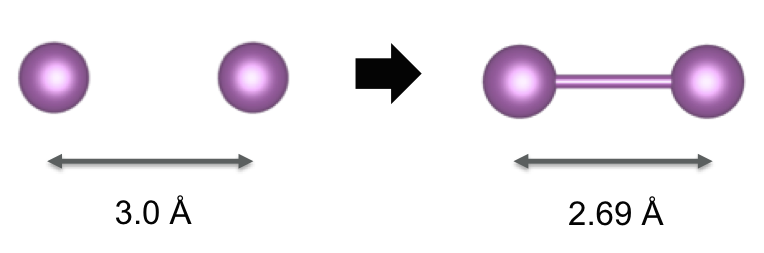
\includegraphics[height=3.5cm]{images/iodine_geom.png}
\caption{Energy minimisation of two iodine atoms from an initial separation of 3.0 \r{A}.}
\label{figure:iodine_dimer}
\end{figure}

\subsection{+U study}

In some DFT studies, an additional potential energy term is sometimes included to better capture the Coulomb interaction of localised electrons. An LDA or GGA functional alone will typically not describe this interaction correctly, especially for localised $d$ and $f$ electrons. Of particular concern is the calculated value of the band gap from DFT simulations, as this value may deviate by up to 30\% from experimental values. Remedying this shortcoming with an appropriate +U parameter could therefore be valuable in obtaining accurate energies. A +U study of the zirconium atom, with an electronic configuration of [Kr]$4d^{2}5s^{2}$, was performed to determine the response to and therefore the viability of an additional potential term for the $d$ electrons.

Figure \ref{Figure:plusubandgap} shows the effect on the calculated band gap when introducing a +U term. While the +U term does increase the band gap, the effect is insignificant. Even with +U terms of 10 eV, the calculated band gap falls short of the experimental band gap by at least 1.5 eV. Moreover, with +U terms greater than 4 eV, we begin to see erratic behaviour in the development of both the band gap, and also in the predicted crystal structure.


%I've got some more information from the +U data below. It looks as though 10 eV might be the point after which we get unusual behaviour. 

%Cubic is fine, it just keeps expanding with +U as we expect. The tetragonal phase expands in the short a&b directions but contracts in the long c direction (i.e. becomes more 'cubic') up until 6 eV, after which it grows in the same manner as cubic.

%The monoclinic phase is harder to explain. There is a cross-over in the length of the a and b parameter at around 4 eV, and then the beta angle (the ~99 deg between a and c) snaps into 90 deg at 11 eV, and when I look at the output structure at this energy, the coordination number of Zr is 6, down from 7. That's why the lattice parameters don't fall into a=b=c, because it doesn't become cubic.

%As you can see from the band gap plot below, just +U by itself is not enough to reproduce the experimental band gap, even for monoclinic. We're off by about 1.5 eV in each case.

\begin{figure}[ht] % +U band gaps
\begin{center}
\begin{tikzpicture}
	\begin{axis}
		[width=11cm, xlabel={+U on Zr \emph{d} orbitals (eV)}, ylabel={Band gap (eV)}, ymin=3.2, ymax=5, xmin=0, xmax=12, legend style={{draw=}, at={(0.35,0.95)}, anchor=north east, legend columns=1}]
		\addplot[no marks] table [x=plusU, y=bandgap,]{dat/plus_u_mono.dat}; \addlegendentry{Monoclinic};
        \addplot[no marks, dashed] table [x=plusU, y=bandgap, ]{dat/plus_u_tet.dat}; \addlegendentry{Tetragonal};
        \addplot[no marks, densely dotted, black] table [x=plusU, y=bandgap,]{dat/plus_u_cubic.dat}; \addlegendentry{Cubic};
			\end{axis}
		\end{tikzpicture}
		\caption{Calculated band gaps for different +U values in monoclinic, tetragonal and cubic \zirconia .}
		\label{Figure:plusubandgap}
	\end{center}
\end{figure}

In monoclinic \zirconia , the use of a +U term causes the lattice parameters to change disproportionately, as seen in Figure \ref{Figure:plusumono}. All lattice parameters increased with larger +U terms, however, expansion in the $a$ direction proceeded faster than in the $b$ direction, resulting in the $a$ lattice parameter becoming larger at a +U of 4 eV. +U terms larger than 10.5 eV caused the lattice parameters to snap suddenly onto new values. A  investigation of the atomic positions revealed that the monoclinic crystal structure had collapsed into an orthorhombic structure, with the co-ordination number of zirconium ions falling to 6 from 7.

\begin{figure} % +U mono
\begin{center}
\begin{tikzpicture}
	\begin{axis}
		[width=11cm, xlabel={+U on Zr \emph{d} orbitals (eV)}, ylabel={Lattice parameter (\r{A})}, ymin=4.9, ymax=6.3, xmin=0, xmax=12, legend style={{draw=}, at={(0.18,0.95)}, anchor=north east, legend columns=1}]
		\addplot[no marks] table [x=plusU, y=a,]{dat/plus_u_mono.dat}; \addlegendentry{$a$};
        \addplot[no marks, dashed] table [x=plusU, y=b, ]{dat/plus_u_mono.dat}; \addlegendentry{$b$};
        \addplot[no marks, densely dotted, black] table [x=plusU, y=c,]{dat/plus_u_mono.dat}; \addlegendentry{$c$};
			\end{axis}
		\end{tikzpicture}
		\caption{Individual lattice parameters as a function of +U term in monoclinic \zirconia .}
		\label{Figure:plusumono}
	\end{center}
\end{figure}

\begin{figure}[ht] % +U tet
\begin{center}
\begin{tikzpicture}
	\begin{axis}
		[width=11cm, xlabel={+U on Zr \emph{d} orbitals (eV)}, ylabel={$a$ parameter (\r{A})}, ymin=3.6, ymax=3.8, xmin=0, xmax=12, legend style={{draw=}, at={(0.18,0.95)}, anchor=north east, legend columns=1}, tick pos=left]
		\addplot[no marks] table [x=plusU, y=a,]{dat/plus_u_tet.dat}; \addlegendentry{$a$};
        %\addplot[no marks, dashed] table [x=plusU, y=b, ]{dat/plus_u_tet.dat}; \addlegendentry{b};
        \addplot[no marks, dashed, black] table [x=plusU, y=c,]{dat/plus_u_tet.dat}; \addlegendentry{$c$};
			\end{axis}
            \begin{axis}[width=11cm,
     xmin = 0, xmax = 12,
     ymin = 5.16, ymax = 5.32,
     hide x axis,
     hide y axis, tick pos=right]
     \addplot[no marks, dashed, black] table [x=plusU, y=c,]{dat/plus_u_tet.dat};
   			\end{axis}
            \pgfplotsset{every axis y label/.append style={rotate=180}}
   \begin{axis}[width=11cm,
         xmin=0, xmax=12,
         ymin=5.16, ymax=5.32,
         hide x axis,
         axis y line*=right,
         ylabel={$c$ parameter (\r{A})}
     ]
   \end{axis}
		\end{tikzpicture}
		\caption{Individual lattice parameters as a function of +U term in tetragonal \zirconia .}
		\label{Figure:plusutet}
	\end{center}
\end{figure}

\begin{figure}[ht] % +U cubic
\begin{center}
\begin{tikzpicture}
	\begin{axis}
		[width=11cm, xlabel={+U on Zr \emph{d} orbitals (eV)}, ylabel={Lattice parameter (\r{A})}, ymin=5.1, ymax=5.35, xmin=0, xmax=12, legend style={{draw=}, at={(0.18,0.95)}, anchor=north east, legend columns=1}]
		\addplot[no marks] table [x=plusU, y=a,]{dat/plus_u_cubic.dat}; \addlegendentry{$a$};
        %\addplot[no marks, dashed] table [x=plusU, y=b, ]{dat/plus_u_cubic.dat}; \addlegendentry{b};
        %\addplot[no marks, densely dotted, black] table [x=plusU, y=c,]{dat/plus_u_cubic.dat}; \addlegendentry{c};
			\end{axis}
		\end{tikzpicture}
		\caption{Individual lattice parameters as a function of +U term in cubic \zirconia .}
		\label{Figure:plusucubic}
	\end{center}
\end{figure}